%%%%%%%% ICML 2021 EXAMPLE LATEX SUBMISSION FILE %%%%%%%%%%%%%%%%%

\documentclass{article}

\usepackage{microtype}
\usepackage{subfigure}
\usepackage{booktabs}
\usepackage[dvips]{graphicx}
\usepackage{multirow,multicol}
\usepackage[table]{xcolor}
\usepackage{listings}
\usepackage{float}
\usepackage[export]{adjustbox}
\usepackage{amssymb}
\usepackage{amsfonts}
\usepackage{amsthm}
\usepackage{amsmath}
\usepackage{enumitem}
\usepackage{lipsum}
\usepackage{pdfpages}
\usepackage{xcolor} 
\usepackage{hyperref}
\usepackage[accepted]{icml2021}


\definecolor{codegreen}{rgb}{0,0.6,0}
\definecolor{codegray}{rgb}{0.5,0.5,0.5}
\definecolor{codepurple}{rgb}{0.58,0,0.82}
\definecolor{backcolour}{rgb}{255,255,255}

\lstdefinestyle{mystyle}{
    backgroundcolor=\color{backcolour},   
    commentstyle=\color{codegreen},
    keywordstyle=\color{magenta},
    numberstyle=\tiny\color{codegray},
    stringstyle=\color{codepurple},
    basicstyle=\ttfamily\footnotesize,
    breakatwhitespace=false,         
    breaklines=true,                 
    captionpos=b,                    
    keepspaces=true,                 
    numbers=left,                    
    numbersep=5pt,                  
    showspaces=false,                
    showstringspaces=false,
    showtabs=false,                  
    tabsize=2
}

\lstset{style=mystyle}

\graphicspath{{./}} 

% Attempt to make hyperref and algorithmic work together better:
%\newcommand{\theHalgorithm}{\arabic{algorithm}}

\begin{document}

\twocolumn[
\icmltitle{Reimplementation of the Classical Neural Ordinary Differential Equation \\
            Using Modern Computational Tools}

\begin{icmlauthorlist}
\icmlauthor{Wasif Ul Islam}{pu}
\end{icmlauthorlist}

\icmlaffiliation{pu}{School of Electrical and Computer Engineering, Purdue University, West Lafayette, Indiana USA}

\icmlkeywords{Machine Learning, ICML}

\vskip 0.3in
]

\printAffiliationsAndNotice{} % otherwise use the standard text.


\section{Introduction}
\label{submission}

Residual Neural Networks (RNN) provided a significant improvement on performance regarding deep
layered neural networks. The performance gains were obtained from introducing residual elements applied
to the ReLu operations within the hidden layer. This introduced robustness against the vanishing/exploding gradient
problem that most classical neural networks face \cite{19Shorten}.

However, there are some application of RNNs that still did not provide the ideal flexibility, in terms
of training models for data involving time-series data. Since RNNs have discrete hidden layers and residual
components to the ReLu operations performed to the hidden layers, it can interfere with learning dependencies
which are sensitive to time \cite{23Walther}.

A different class of neural networks look to satisfy the drawbacks that the previously mentioned network contain:
Neural Ordinary Differential Equations (NeuralODE). The prime benefit that NeuralODEs provide is it is naturally suited for modelling continuos
time data. In addition, it can provide computational flexibility in terms of configurability in forward-pass and backpropagation. 

This paper's objective is to provide a brief literature review into works that have enabled the use of NeuralODEs and discuss the
advantages and disadvantages related to the use of NeuralODEs. As many pieces of work focus on performance of NeuralODEs on time-series datasets,
a short experiment involving the classification of the MNIST dataset using a proof-of-concept NeuralODE model 
is presented along with comparisons of performance with a typical proof-of-concept implementation of a residual neural network.

\section{Related Works}

\subsection{Article: Neural Ordinary Differential Equations}

The concept of NeuralODEs have been discussed before the prescribed implementation by the paper
\textit{Neural Ordinary Differential Equations}. However, the primitive approach to the implementation of
NeuralODEs had very large computational resource consumption, to the point where training the model
on a substantial scale was not feasable. Since the NeuralODE consist of one continous layer with specific time steps
for numerical integration (Derivation of Neural ODE vs. Classical NN is explained further below), performing backpropagation
on NeuralODEs would be taking the gradient across each of the time steps. Since solving ODEs require small timesteps for accurate
representation of the dynamics that is being learned, ordinary back-propagation become as resource dependant as a ResNet with hundreds
of layers.

The major contribution for the respective paper is the adjoint sensitvity method, which allows for the back-propagation of
NeuralODE block at near constant space-complexity \cite{15He}. A comparison between a Recurrent Neural Network with 25
hidden-layers and the proposed NeuralODE architecture was presented with time-series data. 

\begin{figure}[H]
   \centering
   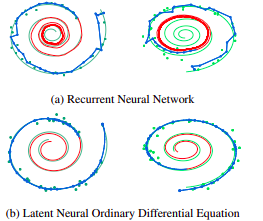
\includegraphics[width=0.75\linewidth]
   {./TimeSeries.png}
   \caption{Comparison Between Recurrent Neural Network and NeuralODE on Time-Series Data \cite{15He}}
   \label{fig:my_label}
\end{figure}

\subsection{Article: Augmented Neural ODE}

The family of NeuralODEs have been extended from the previous contribution to make it more generalizable for existing framworks.
The paper \textit{Augmented Neural ODEs} proposes several postulates. The first assertion is that the classical implementation
of NeuralODEs with the use of adjoint sensitivity method has limitations regarding representation of functions containing intersecting vector flows. The second
assertion involves the existance of output space being rigid to the input space. The proposed solution to the problem was to introduce
higher-dimensionality to the output space. This allows the ODE learning algorithm to lift points into additional dimension without having
differential collisions \cite{19Dupont}. The higher dimensionality mapping allowed for functions that were not representable by the classical
NeuralODEs, available for training.

\begin{figure}[H]
   \centering
   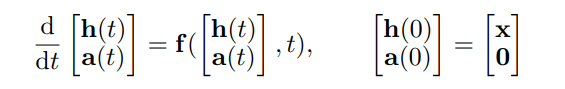
\includegraphics[width=\columnwidth]
   {./Augmented_ODe.png}
   \caption{Activation Function Augmented with Higher Dimensionality \cite{19Dupont}}
   \label{fig:my_label}
\end{figure}


\subsection{Article: How to Train Your Neural ODE}

Beside the adjoint sensitivity method, developed by the authors of the paper \textit{Neural Ordinary Differential Equations},
parallel efforts were also taken to address concerns of high resource usage of back-propagation of NeuralODEs. The paper
\textit{How To Train Your Neural ODE} proposes a method to reduce the computational complexity of back-propagation
in time-series data predictions, by introducing regularization terms to the loss-function \cite{20Finlay}. This allows
for simpler solutions that can be sufficient while limiting NFEs (Number of Function Evaluation) to a reasonable number.
The first regularization term penalty enourages particles to travel with one-dimensional translation by using optimal transport
mapping, while the second regularization term enforces limitations of the vector-field Jacobian to provide force experienced
to be as constant as possible. Such constraint of dynamics allow for simpler solutions with less computational complexities \cite{20Finlay}.

\subsection{A Comparative Derivation of Neural ODE}

Conceptially, NeuralODEs are an extension of Residual Neural Networks. As mentioned previously, the difference between the respective
family of neural networks is the continuos nature of NeuralODEs vs. the discrete nature of Residual Neural Networks. To show the difference,
we will go from one forward-pass calculation of a Residual Neural Network to a NeuralODE.

\textbf{Residual Neural Network}

\[
   h_{t+1} = ReLu(W_{t}h_{t} + b_{t}) + h_{t}
\]

The additional hidden layer term added after the activation function is the residual component of the Residual Neural Network.

Containing the activation function with standard notations, we can rewrite the equation as:

\[
   h_{t} = f(h_{t}, \theta_{t}) + h_{t}
\]

We can convert the following equation to its differential form by expressing it in terms of its limits

\[
   h_{t+1} - h_{t} = f(h_{t}, \theta_{t})
\]

If we reduce the change between one hidden layer to the next to be infinitesimally small, we can express the equation as:

\[
   \frac{h_{t+\delta} - h_{t}}{\delta} = f(h_{t}, \theta_{t})
\]

Taking the limit of $\delta$ and setting it to zero provides us with the differential form of the equation:

\[
   \lim_{\delta \to 0} \hspace*{1ex} \frac{h_{t+\delta} - h_{t}}{\delta} = f(h_{t}, \theta_{t})
\]

\[
   \mathbf{\frac{dh_{t}}{dt} = f(h_{t}, \theta_{t})}
\]

\begin{itemize}
   \item Legend:
   \begin{itemize}
      \item $h_{t}$: Hidden Layer $t$
      \item $W_{t}$: Weight Matrix $t$
      \item $b_{t}$: Bias Vector $t$
      \item $\theta_{t}$: Layer Parameters $t$
      \item $\delta$: Change in Hidden Layer (Infinitesimally Small)
   \end{itemize}
\end{itemize}

\section{Experiment}

\subsection{Defining the Experiment}

An implementation of the Proof-of-Concept NeuralODE is developed. The workflow is modified from a
typical NeuralODE implementation to accomodate visual classification of the MNIST dataset

The paper body should be set in 10~point type with a vertical spacing
of 11~points. Please use Times typeface throughout the text.

\subsection{Title}

The paper title should be set in 14~point bold type and centered
between two horizontal rules that are 1~point thick, with 1.0~inch
between the top rule and the top edge of the page. Capitalize the
first letter of content words and put the rest of the title in lower
case.

\subsection{Author Information for Submission}
\label{author info}

ICML uses double-blind review, so author information must not appear. If
you are using \LaTeX\/ and the \texttt{icml2021.sty} file, use
\verb+\icmlauthor{...}+ to specify authors and \verb+\icmlaffiliation{...}+ to specify affiliations. (Read the TeX code used to produce this document for an example usage.) The author information
will not be printed unless \texttt{accepted} is passed as an argument to the
style file.
Submissions that include the author information will not
be reviewed.

\subsubsection{Self-Citations}

If you are citing published papers for which you are an author, refer
to yourself in the third person. In particular, do not use phrases
that reveal your identity (e.g., ``in previous work \cite{langley00}, we
have shown \ldots'').

Do not anonymize citations in the reference section. The only exception are manuscripts that are
not yet published (e.g., under submission). If you choose to refer to
such unpublished manuscripts \cite{anonymous}, anonymized copies have
to be submitted
as Supplementary Material via CMT\@. However, keep in mind that an ICML
paper should be self contained and should contain sufficient detail
for the reviewers to evaluate the work. In particular, reviewers are
not required to look at the Supplementary Material when writing their
review.

\subsubsection{Camera-Ready Author Information}
\label{final author}

If a paper is accepted, a final camera-ready copy must be prepared.
%
For camera-ready papers, author information should start 0.3~inches below the
bottom rule surrounding the title. The authors' names should appear in 10~point
bold type, in a row, separated by white space, and centered. Author names should
not be broken across lines. Unbolded superscripted numbers, starting 1, should
be used to refer to affiliations.

Affiliations should be numbered in the order of appearance. A single footnote
block of text should be used to list all the affiliations. (Academic
affiliations should list Department, University, City, State/Region, Country.
Similarly for industrial affiliations.)

Each distinct affiliations should be listed once. If an author has multiple
affiliations, multiple superscripts should be placed after the name, separated
by thin spaces. If the authors would like to highlight equal contribution by
multiple first authors, those authors should have an asterisk placed after their
name in superscript, and the term ``\textsuperscript{*}Equal contribution"
should be placed in the footnote block ahead of the list of affiliations. A
list of corresponding authors and their emails (in the format Full Name
\textless{}email@domain.com\textgreater{}) can follow the list of affiliations.
Ideally only one or two names should be listed.

A sample file with author names is included in the ICML2021 style file
package. Turn on the \texttt{[accepted]} option to the stylefile to
see the names rendered. All of the guidelines above are implemented
by the \LaTeX\ style file.

\subsection{Abstract}

The paper abstract should begin in the left column, 0.4~inches below the final
address. The heading `Abstract' should be centered, bold, and in 11~point type.
The abstract body should use 10~point type, with a vertical spacing of
11~points, and should be indented 0.25~inches more than normal on left-hand and
right-hand margins. Insert 0.4~inches of blank space after the body. Keep your
abstract brief and self-contained, limiting it to one paragraph and roughly 4--6
sentences. Gross violations will require correction at the camera-ready phase.

\subsection{Partitioning the Text}

You should organize your paper into sections and paragraphs to help
readers place a structure on the material and understand its
contributions.

\subsubsection{Sections and Subsections}

Section headings should be numbered, flush left, and set in 11~pt bold
type with the content words capitalized. Leave 0.25~inches of space
before the heading and 0.15~inches after the heading.

Similarly, subsection headings should be numbered, flush left, and set
in 10~pt bold type with the content words capitalized. Leave
0.2~inches of space before the heading and 0.13~inches afterward.

Finally, subsubsection headings should be numbered, flush left, and
set in 10~pt small caps with the content words capitalized. Leave
0.18~inches of space before the heading and 0.1~inches after the
heading.

Please use no more than three levels of headings.

\subsubsection{Paragraphs and Footnotes}

Within each section or subsection, you should further partition the
paper into paragraphs. Do not indent the first line of a given
paragraph, but insert a blank line between succeeding ones.

You can use footnotes\footnote{Footnotes
should be complete sentences.} to provide readers with additional
information about a topic without interrupting the flow of the paper.
Indicate footnotes with a number in the text where the point is most
relevant. Place the footnote in 9~point type at the bottom of the
column in which it appears. Precede the first footnote in a column
with a horizontal rule of 0.8~inches.\footnote{Multiple footnotes can
appear in each column, in the same order as they appear in the text,
but spread them across columns and pages if possible.}

\begin{figure}[ht]
\vskip 0.2in
\begin{center}
\centerline{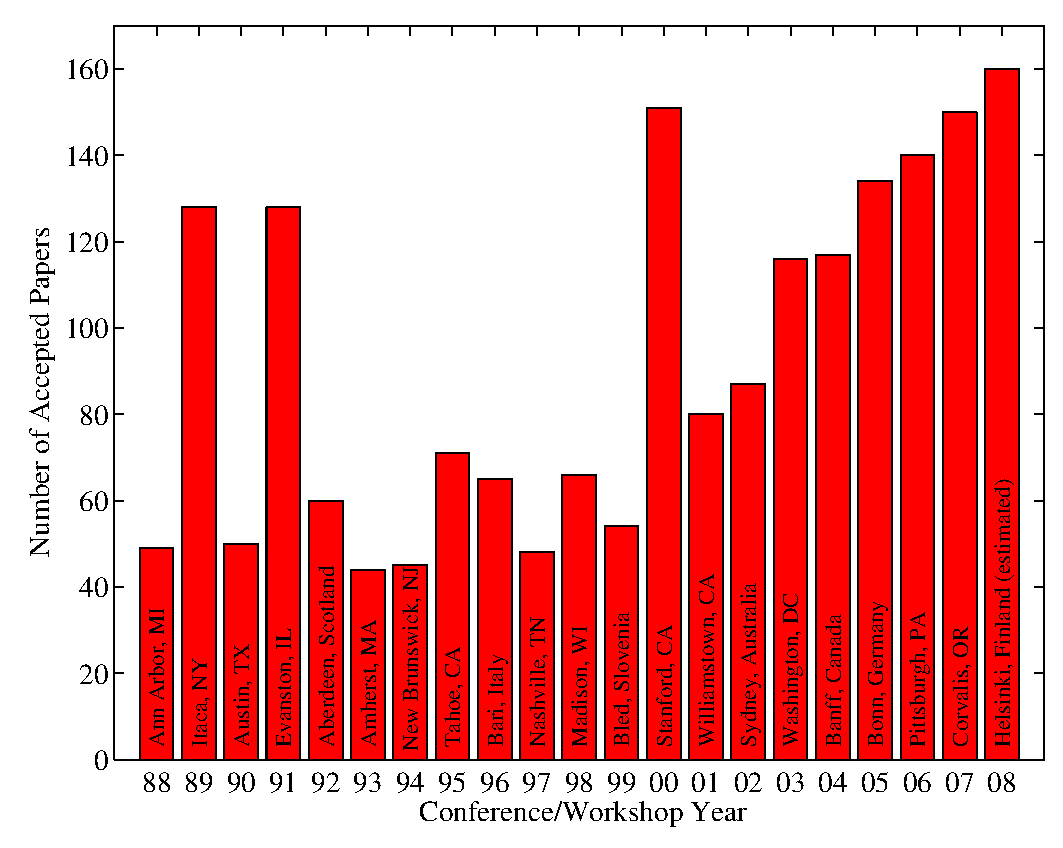
\includegraphics[width=\columnwidth]{icml_numpapers}}
\caption{Historical locations and number of accepted papers for International
Machine Learning Conferences (ICML 1993 -- ICML 2008) and International
Workshops on Machine Learning (ML 1988 -- ML 1992). At the time this figure was
produced, the number of accepted papers for ICML 2008 was unknown and instead
estimated.}
\label{icml-historical}
\end{center}
\vskip -0.2in
\end{figure}

\subsection{Figures}

You may want to include figures in the paper to illustrate
your approach and results. Such artwork should be centered,
legible, and separated from the text. Lines should be dark and at
least 0.5~points thick for purposes of reproduction, and text should
not appear on a gray background.

Label all distinct components of each figure. If the figure takes the
form of a graph, then give a name for each axis and include a legend
that briefly describes each curve. Do not include a title inside the
figure; instead, the caption should serve this function.

Number figures sequentially, placing the figure number and caption
\emph{after} the graphics, with at least 0.1~inches of space before
the caption and 0.1~inches after it, as in
Figure~\ref{icml-historical}. The figure caption should be set in
9~point type and centered unless it runs two or more lines, in which
case it should be flush left. You may float figures to the top or
bottom of a column, and you may set wide figures across both columns
(use the environment \texttt{figure*} in \LaTeX). Always place
two-column figures at the top or bottom of the page.

\subsection{Algorithms}

If you are using \LaTeX, please use the ``algorithm'' and ``algorithmic''
environments to format pseudocode. These require
the corresponding stylefiles, algorithm.sty and
algorithmic.sty, which are supplied with this package.
Algorithm~\ref{alg:example} shows an example.

\begin{algorithm}[tb]
   \caption{Bubble Sort}
   \label{alg:example}
\begin{algorithmic}
   \STATE {\bfseries Input:} data $x_i$, size $m$
   \REPEAT
   \STATE Initialize $noChange = true$.
   \FOR{$i=1$ {\bfseries to} $m-1$}
   \IF{$x_i > x_{i+1}$}
   \STATE Swap $x_i$ and $x_{i+1}$
   \STATE $noChange = false$
   \ENDIF
   \ENDFOR
   \UNTIL{$noChange$ is $true$}
\end{algorithmic}
\end{algorithm}

\subsection{Tables}

You may also want to include tables that summarize material. Like
figures, these should be centered, legible, and numbered consecutively.
However, place the title \emph{above} the table with at least
0.1~inches of space before the title and the same after it, as in
Table~\ref{sample-table}. The table title should be set in 9~point
type and centered unless it runs two or more lines, in which case it
should be flush left.

% Note use of \abovespace and \belowspace to get reasonable spacing
% above and below tabular lines.

\begin{table}[t]
\caption{Classification accuracies for naive Bayes and flexible
Bayes on various data sets.}
\label{sample-table}
\vskip 0.15in
\begin{center}
\begin{small}
\begin{sc}
\begin{tabular}{lcccr}
\toprule
Data set & Naive & Flexible & Better? \\
\midrule
Breast    & 95.9$\pm$ 0.2& 96.7$\pm$ 0.2& $\surd$ \\
Cleveland & 83.3$\pm$ 0.6& 80.0$\pm$ 0.6& $\times$\\
Glass2    & 61.9$\pm$ 1.4& 83.8$\pm$ 0.7& $\surd$ \\
Credit    & 74.8$\pm$ 0.5& 78.3$\pm$ 0.6&         \\
Horse     & 73.3$\pm$ 0.9& 69.7$\pm$ 1.0& $\times$\\
Meta      & 67.1$\pm$ 0.6& 76.5$\pm$ 0.5& $\surd$ \\
Pima      & 75.1$\pm$ 0.6& 73.9$\pm$ 0.5&         \\
Vehicle   & 44.9$\pm$ 0.6& 61.5$\pm$ 0.4& $\surd$ \\
\bottomrule
\end{tabular}
\end{sc}
\end{small}
\end{center}
\vskip -0.1in
\end{table}

Tables contain textual material, whereas figures contain graphical material.
Specify the contents of each row and column in the table's topmost
row. Again, you may float tables to a column's top or bottom, and set
wide tables across both columns. Place two-column tables at the
top or bottom of the page.

\subsection{Citations and References}

Please use APA reference format regardless of your formatter
or word processor. If you rely on the \LaTeX\/ bibliographic
facility, use \texttt{natbib.sty} and \texttt{icml2021.bst}
included in the style-file package to obtain this format.

Citations within the text should include the authors' last names and
year. If the authors' names are included in the sentence, place only
the year in parentheses, for example when referencing Arthur Samuel's
pioneering work \yrcite{Samuel59}. Otherwise place the entire
reference in parentheses with the authors and year separated by a
comma \cite{Samuel59}. List multiple references separated by
semicolons \cite{kearns89,Samuel59,mitchell80}. Use the `et~al.'
construct only for citations with three or more authors or after
listing all authors to a publication in an earlier reference \cite{MachineLearningI}.

Authors should cite their own work in the third person
in the initial version of their paper submitted for blind review.
Please refer to Section~\ref{author info} for detailed instructions on how to
cite your own papers.

Use an unnumbered first-level section heading for the references, and use a
hanging indent style, with the first line of the reference flush against the
left margin and subsequent lines indented by 10 points. The references at the
end of this document give examples for journal articles \cite{Samuel59},
conference publications \cite{langley00}, book chapters \cite{Newell81}, books
\cite{DudaHart2nd}, edited volumes \cite{MachineLearningI}, technical reports
\cite{mitchell80}, and dissertations \cite{kearns89}.

Alphabetize references by the surnames of the first authors, with
single author entries preceding multiple author entries. Order
references for the same authors by year of publication, with the
earliest first. Make sure that each reference includes all relevant
information (e.g., page numbers).

Please put some effort into making references complete, presentable, and
consistent. If using bibtex, please protect capital letters of names and
abbreviations in titles, for example, use \{B\}ayesian or \{L\}ipschitz
in your .bib file.

\section*{Software and Data}

If a paper is accepted, we strongly encourage the publication of software and data with the
camera-ready version of the paper whenever appropriate. This can be
done by including a URL in the camera-ready copy. However, \textbf{do not}
include URLs that reveal your institution or identity in your
submission for review. Instead, provide an anonymous URL or upload
the material as ``Supplementary Material'' into the CMT reviewing
system. Note that reviewers are not required to look at this material
when writing their review.

% Acknowledgements should only appear in the accepted version.
\section*{Acknowledgements}

\textbf{Do not} include acknowledgements in the initial version of
the paper submitted for blind review.

If a paper is accepted, the final camera-ready version can (and
probably should) include acknowledgements. In this case, please
place such acknowledgements in an unnumbered section at the
end of the paper. Typically, this will include thanks to reviewers
who gave useful comments, to colleagues who contributed to the ideas,
and to funding agencies and corporate sponsors that provided financial
support.


% In the unusual situation where you want a paper to appear in the
% references without citing it in the main text, use \nocite
\nocite{langley00}

\bibliography{main}
\bibliographystyle{icml2021}


%%%%%%%%%%%%%%%%%%%%%%%%%%%%%%%%%%%%%%%%%%%%%%%%%%%%%%%%%%%%%%%%%%%%%%%%%%%%%%%
%%%%%%%%%%%%%%%%%%%%%%%%%%%%%%%%%%%%%%%%%%%%%%%%%%%%%%%%%%%%%%%%%%%%%%%%%%%%%%%
% DELETE THIS PART. DO NOT PLACE CONTENT AFTER THE REFERENCES!
%%%%%%%%%%%%%%%%%%%%%%%%%%%%%%%%%%%%%%%%%%%%%%%%%%%%%%%%%%%%%%%%%%%%%%%%%%%%%%%
%%%%%%%%%%%%%%%%%%%%%%%%%%%%%%%%%%%%%%%%%%%%%%%%%%%%%%%%%%%%%%%%%%%%%%%%%%%%%%%
\appendix
\section{Do \emph{not} have an appendix here}

\textbf{\emph{Do not put content after the references.}}
%
Put anything that you might normally include after the references in a separate
supplementary file.

We recommend that you build supplementary material in a separate document.
If you must create one PDF and cut it up, please be careful to use a tool that
doesn't alter the margins, and that doesn't aggressively rewrite the PDF file.
pdftk usually works fine. 

\textbf{Please do not use Apple's preview to cut off supplementary material.} In
previous years it has altered margins, and created headaches at the camera-ready
stage. 
%%%%%%%%%%%%%%%%%%%%%%%%%%%%%%%%%%%%%%%%%%%%%%%%%%%%%%%%%%%%%%%%%%%%%%%%%%%%%%%
%%%%%%%%%%%%%%%%%%%%%%%%%%%%%%%%%%%%%%%%%%%%%%%%%%%%%%%%%%%%%%%%%%%%%%%%%%%%%%%


\end{document}


% This document was modified from the file originally made available by
% Pat Langley and Andrea Danyluk for ICML-2K. This version was created
% by Iain Murray in 2018, and modified by Alexandre Bouchard in
% 2019 and 2021. Previous contributors include Dan Roy, Lise Getoor and Tobias
% Scheffer, which was slightly modified from the 2010 version by
% Thorsten Joachims & Johannes Fuernkranz, slightly modified from the
% 2009 version by Kiri Wagstaff and Sam Roweis's 2008 version, which is
% slightly modified from Prasad Tadepalli's 2007 version which is a
% lightly changed version of the previous year's version by Andrew
% Moore, which was in turn edited from those of Kristian Kersting and
% Codrina Lauth. Alex Smola contributed to the algorithmic style files.
